\documentclass{l4proj}

    
%==============================================================================
% Put any additional packages here
% You can add any packages you want, as long as it does not alter
% the overall format (e.g. don't change the margins or the reference style).
%
\usepackage{pdfpages} % if you want to include a PDF for an ethics checklist, for example
%
%
\usepackage{svg}
\usepackage{wrapstuff}
\usepackage{tikz}
\usepackage{standalone}
\usepackage{pgfplots}
\pgfplotsset{compat=1.15}
\usepackage{mathrsfs}
\usetikzlibrary{arrows}
\newcommand{\degre}{\ensuremath{^\circ}}
\begin{document}

%==============================================================================
%% METADATA
\title{Level 4 Project Report Template} % change this to your title
\author{Pieter van Tuijl}
\date{February 21, 2025}

\maketitle

%==============================================================================
%% ABSTRACT
\begin{abstract}
    Every abstract follows a similar pattern. Motivate; set aims; describe work; explain results.
    \vskip 0.5em
    ``XYZ is bad. This project investigated ABC to determine if it was better.
    ABC used XXX and YYY to implement ZZZ. This is particularly interesting as XXX and YYY have
    never been used together. It was found that
    ABC was 20\% better than XYZ, though it caused rabies in half of subjects.''
\end{abstract}

%==============================================================================
%% ACKNOWLEDGEMENTS
\chapter*{Acknowledgements}
% Enter any acknowledgements here. This is optional; you may leave this blank if you wish,
% or remove the entire chapter
%
% We give thanks to the Gods of LaTeX, who in their eternal graciousness, 
% have granted that this document may compile without errors or overfull hboxes.
%

%==============================================================================

% EDUCATION REUSE CONSENT FORM
% If you consent to your project being shown to future students for educational purposes
% then insert your name and the date below to  sign the education use form that appears in the front of the document. 
% You must explicitly give consent if you wish to do so.
% If you sign, your project may be included in the Hall of Fame if it scores particularly highly.
%
% Please note that you are under no obligation to sign 
% this declaration, but doing so would help future students.
%
%\def\consentname {My Name} % your full name
%\def\consentdate {20 March 2018} % the date you agree
%
\educationalconsent


%==============================================================================
\tableofcontents

%==============================================================================
%% Notes on formatting
%==============================================================================
% The first page, abstract and table of contents are numbered using Roman numerals and are not
% included in the page count. 
%
% From now on pages are numbered
% using Arabic numerals. Therefore, immediately after the first call to \chapter we need the call
% \pagenumbering{arabic} and this should be called once only in the document. 
%
%
% The first Chapter should then be on page 1. 

% PAGE LIMITS
% You are allowed 40 pages for a 40 credit project and 30 pages for a 
% 20 credit report. 
% This includes everything numbered in Arabic numerals (excluding front matter) up
% to but *excluding the appendices and bibliography*.
%
% FORMATTING
% You must not alter text size (it is currently 10pt) or alter margins or spacing.
% Do not alter the bibliography style. 
%
%==================================================================================================================================
%
% IMPORTANT
% The chapter headings and structure here are **suggestions**. You don't have to follow this model if
% it doesn't fit your project. Every project should have an introduction and conclusion,
% however.  If in doubt, your supervisor can give you specific guidance; their view takes precedence over
% the structure suggested here.
%
%==================================================================================================================================
\chapter{Introduction}

% reset page numbering. Don't remove this!
\pagenumbering{arabic}

% You can use \todo{} to mark text that needs to be fixed. Anything inside will appear as highlighted 
% text in the final copy, and you will also get warnings when you compile (so you don't
% forget to take them out!)

\section{Context}

Algorithms drive much of our digital world. They are used in everything from search engines to social media to self-driving cars. Algorithms operate on data and both the data and the operations can be complex and difficult to visualise without good tools. This is particularly the case for spatial data.

Graph data structures are a common way to represent spatial data, where locations are modelled as nodes and connections between the locations as edges. Trees are a type of graph that connect all nodes in a single, connected network. In other words, for each node in the network, there exists exactly one path to all other nodes \citep{tree_graph_theory}.
\\
Here, we will discuss the visualisation of two types of trees: minimum spanning trees and Steiner minimal trees. Additionally, in this project, we only consider the Euclidian variants of these trees. This means that the Euclidian distance between two nodes is used as the edge weight.

\subsection{Minimum Spanning Tree}
A minimum spanning tree (MST) is a tree that connects all nodes in a network with the least amount of total distance.
There exist well-established algorithms for finding the MST of a graph, such as Kruskal's or Prim's algorithm. These algorithms run in polynomial time and work by building up the MST one edge at a time.
\subsection{Steiner Minimal Tree}
A Steiner minimal tree (SMT) is a variant of the MST.
Apart from connecting all nodes in the network with minimal total distance, other nodes may be added to potentially further reduce the total distance. These additional nodes are called Steiner points.
A SMT with zero Steiner points is equivalent to an MST. In contrast to the MST algorithm, finding the optimal SMT is a NP-hard problem, meaning, there exists no polynomial time algorithm for finding the optimal SMT (more on this later).

\colorbox{yellow}{TODO: show example of MST vs SMT}



\section{Aims}
Many tools exist for visualising minimum spanning trees. However, few tools exist for visualising Steiner minimal trees. This is related to the earlier-mentioned fact that the optimal SMT for a given set of nodes is computationally hard to find. This has historically imposed serious limits on the instance sizes that can be solved on an average computer, thus limiting the practicality and usefulness of SMT visualisation tools.
Advances in computer hardware and efficient algorithm implementations, however, have made it possible to solve instances of several orders of magnitude larger than previously possible in reasonable time \citep{29ee725d11ac4584b72f7fe66c4326fa}.

The few existing visualisation tools lack flexibility and a user-friendly interface. (see background)
We aim to fill this gap by developing a user-friendly interface that allows users to visualise SMTs alongside MSTs for graph instances of arbitrary sizes. These instances can be generated randomly or imported from a file.

The interface should be able to display the MST and SMT of a graph simultaneously, allowing for direct comparison of their structures and total length.
\\
Comparison of length will be helpful for building intuition for the \textit{Steiner Ratio},  which is defined as the least upper bound (supremum) of the ratio between the length of the MST and the SMT.  \cite{Gilbert1968SteinerMT} conjectured that this ratio is $$\frac{2}{\sqrt{3}} \approx 1.1547$$
In other words, the \textit{Steiner Ratio} states that the MST is at most 15\% longer than the SMT in the worst case.

Lastly, the interface should be able to dynamically update the solution when the user modifies the graph.

\section{Dissertation Outline}

\colorbox{yellow}{TODO: write at the end of the project}

%- What is this thing/problem about?
%- Why is it important?
%- What is the problem?
%- How is this dissertation going to be structured.



%==================================================================================================================================

\chapter{Background}

\section{Historical context}
The Euclidean Steiner problem has a long history, with roots in the 17th century. The following section will provide a summary of the history as expertly given by \cite{Brazil2014}.

In 1643, Fermat posed the problem of given three points, finding a fourth point such that when connecting the three points to the fourth point, the sum of the distances is minimal. This problem has two cases:
\begin{itemize}
    \item All the interior angles of the triangle formed by the three points are $\le 120^\circ$
    \item One of the interior angles is $\geq 120^\circ$
\end{itemize}

\begin{figure}
    \begin{subfigure}[b]{0.5\textwidth}
        \centering
        \includestandalone[width=\textwidth]{figures/torricelli}
        \caption{Torricelli's and Simpson's constructions for case 1 }
        \label{fig:fermat_1}
    \end{subfigure}
    \hfill
    \begin{subfigure}[b]{0.48\textwidth}
        \centering
        \includestandalone[width=\textwidth]{figures/fermat_2}
        \caption{Case 2 where $\theta \geq 120^\circ$}
        \label{fig:fermat_2}
    \end{subfigure}
    \vskip\baselineskip

    \caption{Solutions to the two cases of Fermat's 3-point problem. \ref{fig:fermat_1} shows two Simpson lines, $EA$ and $DC$, intersecting at the Torricelli point $F$.}
    \label{fig:fermat_problem}
\end{figure}

For the first case, Torricelli proposed the following construction. Given $\triangle ABC$, first draw the equilateral triangles $\triangle ABD$ and $\triangle BCE$. Then, for each of these equilateral triangles, draw the circumcircle. The position where the two circles intersect is the point where the sum of the distances is minimal, the so-called \textit{Torricelli point} (point $F$ in Figure \ref{fig:fermat_1}).
To borrow some terminology from \cite{geosteiner96}, we will call the 3rd point for each of the equilateral triangles an \textit{equilateral point} denoted as $e_{XY}$ where $X$ and $Y$ are the base points from which the equilateral triangle is constructed. So, in figure \ref{fig:fermat_1}, $e_{AB} = D$ and $e_{BC} = E$.

For the second case, Cavalieri proved that the the optimal position of the 4th point is just the point with the obtuse angle. (point $B$ in Figure \ref{fig:fermat_2})

In 1750, Simpson discovered an alternative construction for the first case, where a straight line is drawn from each of the equilateral points to the opposite vertex. The intersection of these lines coincides with the Torricelli point. These "Simpson lines" are demonstrated in Figure \ref{fig:fermat_1}.
Later, in 1834 Heinen proved that a Simpson line has the same length as the sum of the distances to the Torricelli point.

The Fermat-Torricelli problem was later generalised to an $n$-point problem by Gergonne in 1811. Furthermore, Gergonne was also among the first to consider the case where more than one extra point is allowed. He further discovered that there can exist multiple local minimal solutions for the same set of points, and that all have to be constructed in order to find the global minimum. We will return to this concept in the next section.

Another contribution to the problem was made by Gauss in a letter to Schumacher in 1836. He considered the 4-point problem, and noted that using just one extra point does not result in a minimal tree (compare \ref{fig:sub1} with \ref{fig:sub2}) as in the case of the 3-point problem. He went on to illustrate the problem with the example of connecting German cities by railroad with minimal total length.
\begin{quote}
    I have on occasion considered the rail- road connection between Harburg, Bremen, Hannover and Braunschweig, and I myself have thought that this problem would be an excellent prize problem for our students
\end{quote}

The last sentence of the quote proved correct, because two attempts were later made by Bopp in 1879 and Hoffman in 1890 to come up with a solution. Bopp considered all full topologies and used the constructions developed by Gergonne and Simpson to find the Full Steiner Tree (FST) for each full topology (if it exists). Importantly, he generalised the problem to the $n$-point Steiner tree problem and enumerated properties of the Steiner trees, which were later rediscovered and proven by \cite{Gilbert1968SteinerMT}.

Then, in 1934, two Czech mathematicians, Jarník and Kössler, wrote a rigorous treatment on the problem and proved important properties, such as the degree property and the angle property (See \ref{sec:esmt_properties}). They further proved that even if the problem is extended to higher dimensions, the degree and angle properties still hold.

Another 20th-century contribution worth mentioning is the illustration used by Choquet in 1938, where he compares the Steiner tree problem to a network of cities connected by roads where there are no junctions available between the roads except outside the cities. (Another variant is the case where junctions are allowed inside the cities, which is the minimum spanning tree problem). In their influential book \textit{What is Mathematics?}, Courant and Robbins (1941) later used a similar illustration, which they called the "street network problem". Interestingly, they incorrectly attributed the original Fermat-Torricelli problem to Jakob Steiner. As a consequence, the generalised Fermat-Torricelli problem (i.e. the street network problem) has since been known as the Steiner tree problem in the literature despite the fact that Steiner did not originally consider this generalisation.

Finally, \cite{Gilbert1968SteinerMT} provided a comprehensive survey of the Steiner tree problem, and derived many of its properties that have since been the basis for much of the modern literature on the topic. (more on this in \ref{sec:esmt_properties}) From the sixties onwards, the Steiner tree problem has seen a surge in popularity, partly due to the formalisation of computer algorithms for the related minimum spanning tree problem and partly due to real practical applications, such as minimum-length telephone networks and efficient routing in chips. The latter application was presciently predicted by Hanan (1966) in his paper on the rectilinear variant of the Steiner tree problem.

The tool that has been developed as part of this project supports the visualisation of both the Euclidian and rectilinear Steiner minimal trees. The following section will deal with the formal definitions of these two variants and lists some of their properties.
\section{Euclidian Steiner Minimal Tree}

\subsection{Formal definition}
The Euclidian Steiner minimal tree problem is concerned with finding the shortest tree that contains a set of vertices in the Euclidian plane.

More formally:
\begin{itemize}
    \item Let $N$ be a finite set of $n$ points in $\mathbb{R}^2$ (Euclidean plane)
    \item Let $V$ be the set that contains all points in $N$. ($V \supseteq N$)
    \item Let $S = V \setminus N$ be the set of additional points called \textit{Steiner points} where $|S| \geq 0$
    \item Let $T = (V, E)$ be a tree that connects all points in $V$ with exactly $E = |V| - 1$ edges
\end{itemize}

Then, the Euclidian Steiner minimal tree problem seeks to find $T$ such that $\sum_{e \in E} |e|$ is minimised, where $|e|$ is the Euclidean length of edge $e \in E$ \citep{Brazil2014}.

\subsection{Properties}
\label{sec:esmt_properties}
Euclidian Steiner trees have specific properties, which are enumerated in the comprehensive paper by \cite{Gilbert1968SteinerMT}. We list the ones important for our discussion below and refer the reader to the mentioned paper for other properties.
\begin{itemize}
    \item Angle property: every pair of lines meets at $\theta \geq 120^\circ$.
    \item Degree property: every Steiner point has exactly 3 incident edges.
    \item A Steiner tree with $n$ terminals has at most $s \leq n - 2$ Steiner points. Since a tree has $n - 1$ edges, a Steiner tree with $n$ terminals has at most $2n - 3$ edges.
    \item At most one relatively minimal tree exists for a given topology.
    \item A Steiner minimal tree is a union of Full Steiner Trees (FSTs). And every non-full Steiner tree can be decomposed into a union of FSTs.
\end{itemize}

Next, we clarify the following terms, used across the literature and first defined by \cite{Gilbert1968SteinerMT}:
\begin{itemize}
    \item A topology is defined as the adjancy matrix which only specifies the connections between points (i.e. how points are interconnected). \ref{fig:sub4} displays three different topologies for the same set of points, where \ref{fig:sub2} and \ref{fig:sub3} share the same topology.
    \item A full topology has $n - 2$ Steiner points. A Full Steiner Tree (FST) is the relatively minimal tree for a full topology, where the terminals are leaves and the Steiner points are internal nodes with degree 3.
    \item A relatively minimal tree (RMT) is the minimal tree for a given topology. All figures in \ref{fig:grid_figure} are RMTs except for \ref{fig:sub2}. A relatively minimal tree is obtained when small pertubations (displacements) of the Steiner points no longer result in a smaller tree.
    \item  A Steiner tree (ST) is always a RMT, but the converse does not hold. For instance, \ref{fig:sub1} is a RMT but the angle $\angle S_1A_1A_2 = \theta < 120^\circ$ and therefore does not satisfy the angle property.
    \item A Steiner minimal tree (SMT) is a Steiner tree and is minimal for all its vertices (i.e. terminals + Steiner points). In other words, the SMT is the minimal tree across all possible topologies for a given set of points. See Figure \ref{fig:sub4} for an example.
\end{itemize}

Given a topology, its Steiner tree (if it exists) can be seen as a local minimum. Only by enumerating all possible topologies and their corresponding Steiner trees can the global minimum (i.e. the SMT) be found. This concept forms the basis of the algorithms we will discuss in the algorithms section.

\subsection{Steiner ratio}
\label{sec:esmt_steiner_ratio}
An ESMT without Steiner points is equivalent to the Euclidian minimum spanning tree (EMST). Formally, the EMST is defined as the network that connects a set of points $N$, such that the sum of the edge weights is minimal, where the edge weights are the Euclidean distances between the points.

SMTs are shorter or at worst equal in length to MSTs. The ratio between the length of the SMT and the MST has received much attention in the literature. \cite{Gilbert1968SteinerMT} famously conjectured that the lowest possible ratio is $\frac{\sqrt{3}}{2} \approx 0.866025...$ for any set of points.
$$
    \text{Steiner ratio} = \frac{L_{ESMT}}{L_{EMST}} = \frac{\sqrt{3}}{2}
$$

\cite{Steiner_ratio_proof} submitted a proof for this conjecture which was later shown to contain a flaw which invalidated the proof \citep{Steiner_ratio_proof_invalidated}. Hence, the Steiner ratio conjecture remains open to this day.
Nevertheless, attempts have been made to find proofs where $n$ is bounded. For example, \cite{Steiner_ratio_proof_8_points} submitted a proof for the case where $n \leq 8$.


\begin{figure}
    \begin{subfigure}[b]{0.48\textwidth}
        \centering
        \includestandalone[width=\textwidth]{figures/rmt_1}
        \caption{Relatively minimal tree for its topology}
        \label{fig:sub1}
    \end{subfigure}
    \hfill
    \begin{subfigure}[b]{0.48\textwidth}
        \centering
        \includestandalone[width=\textwidth]{figures/rmt_2}
        \caption{Splitting at $A_1$ to add a Steiner point}
        \label{fig:sub2}
    \end{subfigure}
    \vskip\baselineskip
    \begin{subfigure}[b]{0.48\textwidth}
        \centering
        \includestandalone[width=\textwidth]{figures/rmt_3}
        \caption{Steiner tree obtained from \ref{fig:sub2} by perturbing $S_2$ until tree length is minimal for its topology}
        \label{fig:sub3}
    \end{subfigure}
    \hfill
    \begin{subfigure}[b]{0.48\textwidth}
        \centering
        \includestandalone[width=\textwidth]{figures/esmt_1}
        \caption{Steiner minimal tree for all its vertices}
        \label{fig:sub4}
    \end{subfigure}

    \caption{Figures above illustrate how adding and perturbing Steiner points results in increasingly smaller trees. The sub figures a...d are ordered in descending order of tree length. It further shows how the minimal tree for a given topology is not necessarily a Steiner tree, and that a Steiner tree, though minimal for its topology, is not necessarily minimal for all its vertices. b, c, and d are examples of full topologies since they have $n - 2$ Steiner points.}
    \label{fig:grid_figure}
\end{figure}

\section{Rectilinear Steiner Minimal Tree}
\subsection{Formal definition}
The Rectilinear Steiner Minimal Tree (RSMT) problem is similar to the ESMT problem in that by allowing extra Steiner points, it seeks to find the minimal tree for a given set of points, except that the rectilinear distance, also known as the Manhattan distance, is used. The rectilinear distance between two points $p_1 = (x_1, y_1)$ and $p_2 = (x_2, y_2)$ is defined as
$$|x_1 - x_2| + |y_1 - y_2|.$$
\subsection{Properties}
\cite{Brazil2015} provides a list of properties of rectilinear Steiner trees including:
\begin{itemize}
    \item Degree property: every Steiner point $s$ has exactly 3 or 4 incident edges. A Steiner point of degree 3 is called a \textit{T-point}, whilst a Steiner point of degree 4 is called a \textit{cross}.
    \item Every edge has at most 1 horizontal and 1 vertical segment. An edge with exactly 1 horizontal and 1 vertical component is called a \textit{bent edge} whilst an edge with only 1 horizontal component or 1 vertical component is called a \textit{straight edge}.
    \item If $s$ is a T-point, at most one of its incident edges is a bent edge. If $s$ is a cross, then all of its incident edges are straight edges.
\end{itemize}

\subsection{Steiner ratio}
As before, a RSMT without Steiner points is equivalent to a rectilinear minimum spanning tree (RMST). The definition of the RMST is similar to the definition of the ESMT in \ref{sec:esmt_steiner_ratio} except that the rectilinear metric is used.

The Steiner ratio in the rectilinear case is the smallest ratio between the length of the RSMT and the RMST. It has been proven to be exactly $2/3$ \cite{Brazil2015}.
$$
    \text{Steiner ratio} = \frac{L_{RSMT}}{L_{RMST}} = \frac{2}{3}
$$

In other words, the rectilinear minimum spanning tree is at most 1.5 times the length of the rectilinear Steiner minimal tree.

\section{Algorithms}
The Steiner tree problem is easy to understand but hard to actually solve. \cite{Garey1977} proved that the Euclidian and Rectilinear Steiner tree problems are NP-hard. This means that there exist no polynomial-time algorithms for these problems (unless P = NP).
However, approximation schemes can be used to find near-optimal solutions in a reasonable amount of time. In this project, however, we have chosen to use exact algorithms, in order to demonstrate that despite the hardness of the problem in theory, the actual performance in practise is suprisingly good.

There exists two main exact algorithms for the Steiner tree problem:
\begin{itemize}
    \item The (naive) Melzak algorithm \cite{MelzakAlgo}.
    \item The efficient Geosteiner algorithm developed by \cite{geosteiner96}, which is based on the Melzak algorithm.
\end{itemize}

\subsection{The Melzak (naive) algorithm}
As mentioned at the end of \ref{sec:esmt_properties} there can exists local minimal solutions for the Steiner tree problem. Hence, in order to find the global minimal solution, we need to consider all possible full (Steiner) topologies. The Melzak algorithm does not explicitly deal with this, but assumes an existing full topology and finds the relatively minimal Steiner tree if it exists. We will later see how to generate all full topologies for a given set of points.



The proof in \citep{Garey1977} is very technical so we attempt to give a more intuitive, non-rigorous explanation based on the workings of the naive algorithm.
\subsection{The Melzak (naive) algorithm}

\section{Existing visualisation tools}

During the research phase, we found three related projects on Github whose features and limitations will be discussed in this section.

\subsection{Steiner-Tree-Visualisation (STV)}
STV is a Python-based GUI tool developed by \cite{Steiner-Tree-Visualisation}. It provides a simple interface for visualising Euclidian MSTs and SMTs, displaying their lengths and allowing for direct comparison. However, the tool is limited by a few factors.
\begin{itemize}
    \item First, a brute-force approximation algorithm is used to find the SMT, and despite the ${O(n^4 \log(n))}$ complexity, the tool freezes for instances larger than 40 nodes.
    \item Additionally, the GUI is not very flexible. For example, you cannot overlay the MST and SMT simultaneously and the canvas does not support zooming or resizing. It is also not possible to import a graph from an external file or export the results.
    \item Lastly, the tool does not work out of the box and requires code patching to run in modern Python environments.
\end{itemize}

\subsection{ESteiner-3D (E3D)}
E3D is another Python-based tool developed by \cite{ESteiner-3D}. It is a program that can be used to find the Euclidian SMT of a graph and supports 2D and 3D graphs. However, use of the software is limited by the fact that no graphical nor command-line interface is provided. It also does not support the simultaneous visualisation of MSTs and SMTs and the visualisation of the Steiner ratio.

\subsection{Steiner-Tree (ST)}
ST is a Javascript-based tool developed by \cite{Steiner-Tree}. It is a web page that can be used to find the Rectilinear SMT of a graph. Although the tool has a nice interface and uses an interactive canvas, it does not support visualisation of the MST or SMT in the Euclidian plane. And even for the rectilinear case, it is only possible to place the nodes on grid lines instead of anywhere on the canvas. This makes it possible to use a polynomial-time algorithm, but it makes the tool unsuitable for imported graph instances. Exporting the visualisation results is also not possible.

Overall, we have found that the existing tools are limited by a lack of smooth, user-friendly interfaces, visualisation options, flexible import/export capabilities, and platform independence.

\chapter{Analysis/Requirements}
What is the problem that you want to solve, and how did you arrive at it?
\section{Guidance}
Make it clear how you derived the constrained form of your problem via a clear and logical process.

The analysis chapter explains the process by which you arrive at a concrete design. In software
engineering projects, this will include a statement of the requirement capture process and the
derived requirements.

In research projects, it will involve developing a design drawing on
the work established in the background, and stating how the space of possible projects was
sensibly narrowed down to what you have done.

%==================================================================================================================================
\chapter{Implementation}
Having given a high-level design of the proposed solution in the previous chapter, this chapter will discuss the practicalities of our implementation and address topics such as:
\begin{itemize}
    \item Why we chose to build a web app over a native app.
    \item What tech stack we used and why.
    \item What the big picture architecture is and how different parts are connected.
    \item How the codebase is structured, in order to support extensibility and maintainability.
    \item How we implemented the algorithms and integrated them with the UI, including a in-depth look at the use of WebAssembly (WASM).
\end{itemize}

\section{Building for the web}
The first implementation decision was to build a web app instead of a native app. As stated in the problem description, our aim was to make a visually-appealing and accessible tool that does not require technical expertise or custom tooling for use. Browsers are ubiquitous nowadays and provide a platform-independent way to run and distribute applications. Updates can easily be deployed without the need for users to install them manually.
Futhermore, differences between browser vendors have become less pronounced due to the development of standards and the rise of frameworks that abstract away some of the most jarring differences.

% The constraining factor for web apps has been the performance of computationally intensive tasks. However, this has been mitigated by the development of WebAssembly (WASM), a technology that allows for near-native performance while still being platform-independent.

\subsection{Tech stack}

The application is built using Typescript\footnote{https://www.typescriptlang.org/} (TS) as the main programming language, which is a statically-typed superset of Javascript (JS) that compiles to JS \citep{typescript}.
JS, the web's main language, is dynamically typed and has some loose features that can make it prone to bugs. For example, invalid references are not detected until runtime, in contrast to TS which adds compile-time type checking.
Empirical evidence has shown that TS is effective at detecting bugs and improving code maintainability \citep{typescript_bugs_paper}.

Interactive web applications often rely on something called DOM manipulation. This is the process of mutating HTML elements in the DOM, the tree of HTML elements that make up the UI. DOM manipulation is costly and is a major performance bottleneck for web apps.
We have used React\footnote{https://react.dev/} (which makes use of a virtual DOM) to build an interactive UI whilst still ensuring that the real DOM gets mutated as little as possible.
Moreover, React code is declarative (i.e. we tell what the UI should look like, not how to achieve it) and therefore easier to reason about and maintain.

Other dependencies include:
\begin{itemize}
    \item Shadcn/ui\footnote{https://ui.shadcn.com/} for base UI components, such as buttons, inputs, dropdowns, etc.
    \item Sigma.js\footnote{https://sigmajs.org/} for drawing graphs on the canvas.
    \item Graphology\footnote{https://graphology.github.io/} for the graph data model
\end{itemize}

\subsection{Application architecture}
% See \ref{fig:architecture} for the architecture diagram.
The application has been developed as a client-only application, with no need for a backend API. Figure \ref{fig:architecture} shows the various high-level components of the application. The top-layer (i.e. the frontend) is divided into three main parts:
\begin{itemize}
    \item The views part, which handles user interaction (controls) and the visual appearance
    \item The algorithms part, which handles the computation of the algorithms supported by the application.
    \item The graph datastructure as a global state, which can be read and mutated by the views and algorithms.
\end{itemize}

\begin{figure}[h]
    \centering
    \includesvg[width=0.8\linewidth]{images/architecture_diagram.svg}
    \caption{Architecture of the application. The arrows indicate the flow of data and control.}
    \label{fig:architecture}
\end{figure}

The controls allow the user to modify the graph instance, either directly by adding a new graph or by editing the existing one, or indirectly by triggering the computation of an algorithm.
Updates to the graph datastructure are reflected in the the canvas component.

The lower layer contains the WebAssembly module that contains the WASM byte code of the compiled Geosteiner C-library, which is used for computing the Euclidian and Rectilinear variants of the Steiner minimal tree. The WebAssembly module is dynamically imported by the frontend during runtime.
We discuss the use of WebAssembly in more detail in section \ref{sec:webassembly}.

\section{Algorithm implementations}

\begin{wrapstuff}[r,width=0.3\textwidth,type=figure]
    \centering
    \caption{Interface of the algorithm computational output.}
    \includesvg[width=1\textwidth]{images/algorithm_output.svg}
    \label{fig:algorithm_interface}
\end{wrapstuff}
Each algorithm is implemented as an isolated, pure function that takes an undirected graph as input and returns a computation.
Figure \ref{fig:algorithm_interface} specifies the interface of the computational output. The tree is returned as new graph instance, alongside the length of the tree. The list of edge mutations keeps track of all the edges that were added to the tree in order of insertion. Some algorithms, such as the ESMT and the RSMT also pass additional metadata, such as the list of Steiner nodes.
By coding to an interface as opposed to a concrete implementation, algorithm implementations can be swapped out and new algorithms can be added easily.

The output from the algorithm is used to update the global graph datastructure by a \textit{merge} operation. We can't directly mutate the global graph because of limitations in Sigma.js (the library used for canvas drawing).
Merging the tree with the existing graph is done by adding all the tree edges and nodes into the existing graph. If an edge or node already exists, its attributes are updated to indicate that it is part of the algorithm-generated tree. By keeping track of which edges/nodes are generated by which algorithm, we can toggle the visibility of each tree separately whilst still using the same graph instance.

\wrapstuffclear
\subsection{Euclidian Minimum Spanning Tree}
The EMST is implemented using Prim's algorithm \citep[pp. 194--195]{Skiena2008}. Since the algorithm operates in Euclidian space, the input graph is first preprocessed to be a complete undirected graph. See pseudocode \ref{alg:emst} for the implementation.

\begin{algorithm}
    \caption{Prim's $O(n^2)$ algorithm for the EMST}
    \label{alg:emst}
    \SetAlgoLined
    \KwIn{Graph $G = (V, E)$}
    \KwOut{Tree $T = (V', E')$}
    \SetKwFunction{Prim}{Prim}
    initialize tree $T$, parent vector $p$, distance vector $d$\;
    Set $v$ to startNode\;
    \While{$v$ not in $T$}{
        E = v.edges()\;
        \ForEach{edge $e \in E$}{
            $u \leftarrow$ edge.target()\;
            $w \leftarrow$ edge.weight()\;
            \If{distance[$u$] > $w$ and $u$ not in $T$}{
                distance[$u$] = $w$\;
                parent[$u$] = $v$\;
            }
        }
        $fringe$ = $V \setminus V'$\;
        $v$ = node $u$ in $fringe$ with smallest distance to $v$\;
        T.addNode($v$)\;
        T.addEdge(p[$v$], $v$)\;
    }
    \Return{$T$}\;
\end{algorithm}

\subsection{Euclidean \& Rectilinear Steiner Minimal Tree}
For the ESMT and RSMT, we make use of the Geosteiner\footnote{http://www.geosteiner.com/} C-library implementation. As highlighted in the background section, efficient exact SMT algorithms are hard to implement and the GeoSteiner library is a well-established library that makes use of many heuristics and clever techniques to find the exact solution in a reasonable time.
From the frontend perspective therefore, we treat the library as a black box and only care about the input and the output, whilst leaving the implementation details to the library.

We have implemented a wrapper around the library that provides a simplified interface, only exposing the functions that are needed by the frontend. Listing \ref{lst:wrapper_functions} shows the wrapper functions that are exposed to the frontend.

\begin{lstlisting}[language=C,caption=Wrapper functions for the Geosteiner library,label=lst:wrapper_functions]
      void calc_esmt(int n, double *terms, double *length, int *nsps, double *sps, int *nedges, int *edges);

      void calc_rsmt(int n, double *terms, double *length, int *nsps, double *sps, int *nedges, int *edges);
\end{lstlisting}

The browser, however, cannot execute C code directly. Therefore, we need to compile the C code to WebAssembly (WASM) byte code. We do this using the Emscripten\footnote{https://emscripten.org/} toolchain.
We discuss the details of the compilation process and integration of the WASM module with the frontend in section \ref{sec:webassembly}.

With WASM, we have to explicitly manage memory allocation and deallocation. From the properties of the Steiner minimum tree, we know that the maximum number of Steiner points is $n - 2$ and the maximum number of edges is $2n - 3$. Using these constraints, we pre-allocate the memory for the Steiner points and edges and pass the pointers to the wrapper functions defined above.


\section{WebAssembly}
\label{sec:webassembly}
Previously, Javascript was the only language that could run in the browser. This meant that native code could not be executed and always had to be manually ported to JS.
This limitation let to attempts to compile native code to JS, such as ASM.js. It was found that ASM.js was more performant than code that had been manually rewritten in JS \citep{WebAssemblyIntro}.
In 2015, WebAssembly\footnote{https://webassembly.org/} (WASM) was introduced as new compilation target for the browser. WASM is a binary instruction format that is more performant than JS and can be used to run native code at near native speeds.
WASM is supported by most browsers, with the exception of Internet Explorer and Opera Mini \footnote{https://caniuse.com/wasm}.

WASM is designed to be portable (i.e. write once, run everywhere), similar to C in a sense. Code compiled to WASM can run on any platform, both web and off-web (e.g. Node.js).
The current application is a client-only application, but if we were to decide to run the Geosteiner algorithms on a Node.js backend, WASM would allow us to do so seamlessly.

\subsection{How WASM works}
The browser features a virtual machine (VM) that can execute JS and WASM binary code. A WASM binary is called a module and can be loaded into the VM by calling the WebAssembly Browser APIs from a JS script.
In order for JS to call WASM functions, the WASM module must explicitly export these functions. WASM itself only supports 4 basic data types: 32/64 bit ints/floats. This means that we can't pass complex data structures to a WASM function or return such data from it.
Instead, we can utilise the shared contiguous memory space between JS and WASM to pass pointers to memory locations that contain the data.

\subsection{Emscripten}

As highlighted in the figure \ref{fig:architecture}, the Geosteiner library is compiled to WASM using the Emscripten toolchain. The Emscripten toolchain consists of a designated compiler frontend (emcc) and LLVM backend optimised for the generation of WASM binaries.
Apart from the compiler, the toolchain also exposes a set of "glue code" that aims to simplify the boilerplate code required to both load the WASM module and interface between the WASM module and JS code \citep{Emscripten_tutorial}.

The glue code also provides an ergonomic memory management API. We can 'view' the same memory buffer in different ways depending on the data type, such as an array of 32-bit integers or 64-bit floats. This avoids the need to manually handle different offsets and strides when accessing the data.

The output from the Empscripten compiler is a .wasm file and a .js file. The .js file is imported by the frontend and contains the glue code and is used to asynchronously load and instantiate the WASM module.

\section{Structure of the codebase}

\section{Visualisation/design}

\section{Summary}


%==================================================================================================================================
\chapter{Evaluation}
How good is your solution? How well did you solve the general problem, and what evidence do you have to support that?

\section{Guidance}
\begin{itemize}
    \item
          Ask specific questions that address the general problem.
    \item
          Answer them with precise evidence (graphs, numbers, statistical
          analysis, qualitative analysis).
    \item
          Be fair and be scientific.
    \item
          The key thing is to show that you know how to evaluate your work, not
          that your work is the most amazing product ever.
\end{itemize}

\section{Evidence}
Make sure you present your evidence well. Use appropriate visualisations,
reporting techniques and statistical analysis, as appropriate. The point is not
to dump all the data you have but to present an argument well supported by evidence gathered.

If you use numerical evidence, specify reasonable numbers of significant digits; don't state ``18.41141\% of users were successful'' if you only had 20 users. If you average \textit{anything}, present both a measure of central tendency (e.g. mean, median) \textit{and} a measure of spread (e.g. standard deviation, min/max, interquartile range).

You can use \texttt{siunitx} to define units, space numbers neatly, and set the precision for the whole LaTeX document.

% setup siunitx to have two decimal places
\sisetup{
    round-mode = places,
    round-precision = 2
}

For example, these numbers will appear with two decimal places: \num{3.141592}, \num{2.71828}, and this one will appear with reasonable spacing \num{1000000}.



If you use statistical procedures, make sure you understand the process you are using,
and that you check the required assumptions hold in your case.

If you visualise, follow the basic rules, as illustrated in Figure \ref{fig:boxplot}:
\begin{itemize}
    \item Label everything correctly (axis, title, units).
    \item Caption thoroughly.
    \item Reference in text.
    \item \textbf{Include appropriate display of uncertainty (e.g. error bars, Box plot)}
    \item Minimize clutter.
\end{itemize}

See the file \texttt{guide\_to\_visualising.pdf} for further information and guidance.

\begin{figure}[htb]
    \centering
    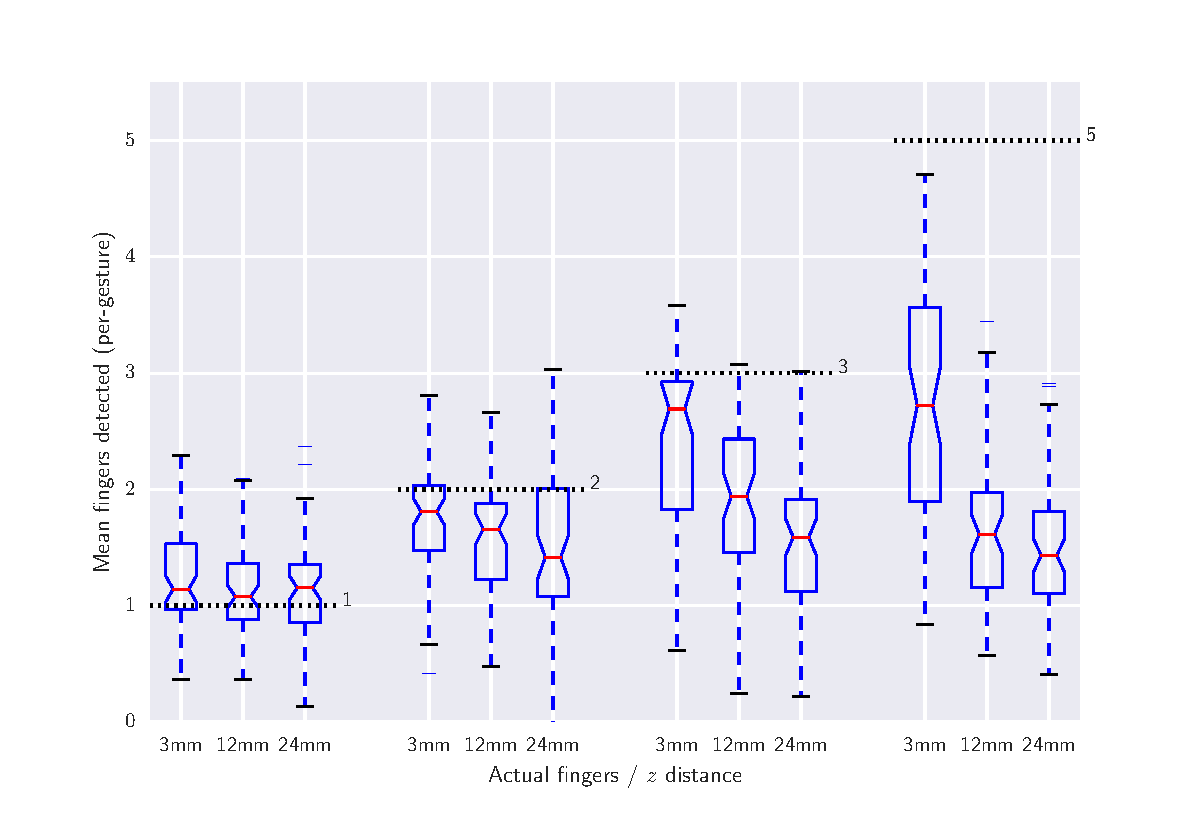
\includegraphics[width=1.0\linewidth]{images/boxplot_finger_distance.pdf}

    \caption{Average number of fingers detected by the touch sensor at different heights above the surface, averaged over all gestures. Dashed lines indicate
        the true number of fingers present. The Box plots include bootstrapped uncertainty notches for the median. It is clear that the device is biased toward
        undercounting fingers, particularly at higher $z$ distances.
    }

    % use the notation fig:name to cross reference a figure
    \label{fig:boxplot}
\end{figure}


%==================================================================================================================================
\chapter{Conclusion}
Summarise the whole project for a lazy reader who didn't read the rest (e.g. a prize-awarding committee). This chapter should be short in most dissertations; maybe one to three pages.
\section{Guidance}
\begin{itemize}
    \item
          Summarise briefly and fairly.
    \item
          You should be addressing the general problem you introduced in the
          Introduction.
    \item
          Include summary of concrete results (``the new compiler ran 2x
          faster'')
    \item
          Indicate what future work could be done, but remember: \textbf{you
              won't get credit for things you haven't done}.
\end{itemize}

\section{Summary}
Summarise what you did; answer the general questions you asked in the introduction. What did you achieve? Briefly describe what was built and summarise the evaluation results.

\section{Reflection}
Discuss what went well and what didn't and how you would do things differently if you did this project again.

\section{Future work}
Discuss what you would do if you could take this further -- where would the interesting directions to go next be? (e.g. you got another year to work on it, or you started a company to work on this, or you pursued a PhD on this topic)

%==================================================================================================================================
%
% 
%==================================================================================================================================
%  APPENDICES  

\begin{appendices}

    \chapter{Appendices}

    Use separate appendix chapters for groups of ancillary material that support your dissertation.
    Typical inclusions in the appendices are:

    \begin{itemize}
        \item
              Copies of ethics approvals (you must include these if you needed to get them)
        \item
              Copies of questionnaires etc. used to gather data from subjects. Don't include
              voluminous data logs; instead submit these electronically alongside your source code.
        \item
              Extensive tables or figures that are too bulky to fit in the main body of
              the report, particularly ones that are repetitive and summarised in the body.
        \item Outline of the source code (e.g. directory structure),
              or other architecture documentation like class diagrams.
        \item User manuals, and any guides to starting/running the software.
              Your equivalent of \texttt{readme.md} should be included.

    \end{itemize}

    \textbf{Don't include your source code in the appendices}. It will be
    submitted separately.



\end{appendices}

%==================================================================================================================================
%   BIBLIOGRAPHY   

% The bibliography style is agsm (Harvard)
% The bibliography always appears last, after the appendices.

\bibliographystyle{agsm}

% Force the bibliography not to be numbered
\renewcommand{\thechapter}{0}
\bibliography{l4proj}

\end{document}
